% VOSS manuscript, first draft. IEEE Transactions format (IEEEtran, journal mode).
% Numbers and tables come from generated/ (python -m experiments.paper_tex); figures from figures/ (experiments.paper_figs).
\documentclass[journal]{IEEEtran}

\usepackage[T1]{fontenc}
\usepackage{amsmath,amssymb}
\usepackage{booktabs}
\usepackage{graphicx}
\usepackage{microtype}
\usepackage{xcolor}
\usepackage{tikz}
\usetikzlibrary{arrows.meta,positioning,shapes.geometric,fit,calc}
\usepackage[hidelinks]{hyperref}
\usepackage{cite}

% Generated by experiments/paper_tex.py from paper/ and configs/calibration/; do not edit.
\newcommand{\AblGeoExp}{34}
\newcommand{\AblGeoP}{0.09}
\newcommand{\AblHedgeP}{0.3}
\newcommand{\AblLifecycleP}{3.3}
\newcommand{\AblNoProgSucc}{1.8}
\newcommand{\AblPlanningExp}{31}
\newcommand{\AblPlanningP}{1.1}
\newcommand{\AblRepExp}{19}
\newcommand{\AblRobustExp}{24}
\newcommand{\AblRobustP}{0.8}
\newcommand{\AlwaysWastePct}{10.6}
\newcommand{\BhDetectHb}{60}
\newcommand{\BhDetectProg}{4.2}
\newcommand{\BhTimeoutsHb}{132}
\newcommand{\BhTimeoutsProg}{0.7}
\newcommand{\CalAttested}{44}
\newcommand{\CalAttestedN}{9}
\newcommand{\CalCpu}{Intel Core i3-7020U}
\newcommand{\CalFcBootColdS}{1.45}
\newcommand{\CalFcBootWarmMs}{154}
\newcommand{\CalQuote}{0.51}
\newcommand{\CalQuotePh}{0.25}
\newcommand{\CalReboot}{21}
\newcommand{\CalRebootPh}{15}
\newcommand{\CalRestoreColdS}{0.63}
\newcommand{\CalRestoreWarmMs}{7}
\newcommand{\CalSensSimplePNinetynineMeas}{4.6}
\newcommand{\CalSensSimplePNinetyninePlc}{3.9}
\newcommand{\CalSensVossPNinetynineMeas}{1.17}
\newcommand{\CalSensVossPNinetyninePlc}{1.32}
\newcommand{\CalShaMBps}{269}
\newcommand{\CalSnapCreate}{6.7}
\newcommand{\CalUserspace}{31}
\newcommand{\CalVerifyMs}{40}
\newcommand{\CommCostForty}{5}
\newcommand{\CommCostRef}{12}
\newcommand{\CommCostTen}{20}
\newcommand{\CommCostTwenty}{10}
\newcommand{\CommPFiftyPct}{45}
\newcommand{\CommPNinetyninePct}{14}
\newcommand{\CrashDetectProg}{2.2}
\newcommand{\CrashFailover}{2.7}
\newcommand{\ExpFOne}{19}
\newcommand{\ExpFTwo}{24}
\newcommand{\ExpFZero}{13}
\newcommand{\FzeroSuccDelta}{0.11}
\newcommand{\GeoClusters}{9}
\newcommand{\GeoExpRatio}{5.1}
\newcommand{\GreedyKeepHigh}{57}
\newcommand{\GreedyKeepMed}{27}
\newcommand{\GreedyNoneHigh}{59}
\newcommand{\GreedyNoneMed}{54}
\newcommand{\GreedySolveMs}{8}
\newcommand{\HEightPct}{8.1}
\newcommand{\HElevenPct}{64}
\newcommand{\HFTOnePct}{3.2}
\newcommand{\HFTOneSuccHb}{96.8}
\newcommand{\HOnePctKeepHigh}{60}
\newcommand{\HOnePctKeepMed}{29}
\newcommand{\HOnePctNoneHigh}{63}
\newcommand{\HOnePctNoneMed}{54}
\newcommand{\HSevenEu}{17}
\newcommand{\HSevenEuNa}{17}
\newcommand{\HSevenWorld}{5}
\newcommand{\HSixPct}{3}
\newcommand{\HTenPct}{1.5}
\newcommand{\HbOmitRatio}{9}
\newcommand{\HbSuccAlpha}{96.8}
\newcommand{\HedgeOffWastePct}{0.5}
\newcommand{\HedgePNinetynineHi}{1}
\newcommand{\HedgePNinetynineLo}{-32}
\newcommand{\HedgePNinetyninePct}{13}
\newcommand{\MilpGreedyHigh}{8.1}
\newcommand{\MilpGreedyHighBelow}{above}
\newcommand{\MilpGreedyHighBest}{21}
\newcommand{\MilpGreedyHighWorst}{1}
\newcommand{\MilpGreedyMed}{1.8}
\newcommand{\MilpGreedyMedBelow}{below}
\newcommand{\MilpGreedyMedBest}{5}
\newcommand{\MilpGreedyMedWorst}{1}
\newcommand{\MilpSolveS}{4.1}
\newcommand{\MilpWarmRatio}{2.1}
\newcommand{\ParetoExpMax}{25}
\newcommand{\ParetoExpMin}{11}
\newcommand{\ParetoFrontN}{3}
\newcommand{\ParetoHighMax}{1.8}
\newcommand{\ParetoKneeExpSaved}{25}
\newcommand{\ParetoKneeF}{0.1}
\newcommand{\ParetoKneePNinetynineLoss}{1.6}
\newcommand{\ParetoLowMax}{1.4}
\newcommand{\ParetoPNinetynineHi}{1.35}
\newcommand{\ParetoPNinetynineLo}{1.27}
\newcommand{\PrecisionMixed}{97}
\newcommand{\RecvKBs}{4.5}
\newcommand{\RecvLatSixty}{30}
\newcommand{\RecvLatTen}{6}
\newcommand{\RecvLatThreeHundred}{118}
\newcommand{\RecvMissingMax}{1}
\newcommand{\RecvRows}{17}
\newcommand{\RecvRuns}{100}
\newcommand{\RecvSettleMs}{14}
\newcommand{\RecvUnexplained}{0}
\newcommand{\RecvVerifyMs}{0.8}
\newcommand{\RepGini}{0.93}
\newcommand{\RepPNinetyninePct}{2.4}
\newcommand{\RepStarved}{65}
\newcommand{\RepTopTen}{93}
\newcommand{\RouteLeastMet}{0.911}
\newcommand{\RouteLeastPNinetynine}{1.39}
\newcommand{\RouteNearMet}{0.991}
\newcommand{\RouteNearPNinetynine}{1.20}
\newcommand{\RpWastePct}{1.8}
\newcommand{\ScaleBigDecide}{30}
\newcommand{\ScaleBigPNinetynine}{28}
\newcommand{\ScaleBigSucc}{81}
\newcommand{\ScaleMidDecide}{14}
\newcommand{\ScaleMidPNinetynine}{16}
\newcommand{\ScaleMidSucc}{97}
\newcommand{\ScaleMsgHi}{1.08}
\newcommand{\ScaleMsgLo}{0.70}
\newcommand{\ScaleTenKSucc}{99.8}
\newcommand{\ScoreInconclusive}{6}
\newcommand{\ScoreRefuted}{5}
\newcommand{\ScoreSupported}{11}
\newcommand{\ScoreWeak}{2}
\newcommand{\SimApplSession}{19}
\newcommand{\SimCocoSession}{8.1}
\newcommand{\SimCvmSession}{1.4}
\newcommand{\SimCvmZeroStart}{2.3}
\newcommand{\SimpleExpRatio}{1.9}
\newcommand{\SlowFailover}{14}
\newcommand{\ViabACells}{9}
\newcommand{\ViabAMetBase}{0}
\newcommand{\ViabAMetBetter}{0}
\newcommand{\ViabAMetNone}{9}
\newcommand{\ViabAMetNoneFive}{0}
\newcommand{\ViabAMetOnly}{9}
\newcommand{\ViabAPFiveBase}{0}
\newcommand{\ViabAPFiveVoss}{9}
\newcommand{\ViabAPThreeBase}{0}
\newcommand{\ViabAPThreeBaseAny}{0}
\newcommand{\ViabAPThreeVoss}{9}
\newcommand{\ViabBCells}{16}
\newcommand{\ViabBMetBase}{4}
\newcommand{\ViabBMetBetter}{2}
\newcommand{\ViabBMetNone}{16}
\newcommand{\ViabBMetNoneFive}{1}
\newcommand{\ViabBMetOnly}{9}
\newcommand{\ViabBPFiveBase}{0}
\newcommand{\ViabBPFiveVoss}{16}
\newcommand{\ViabBPThreeBase}{0}
\newcommand{\ViabBPThreeBaseAny}{0}
\newcommand{\ViabBPThreeVoss}{13}
\newcommand{\ViabCCells}{12}
\newcommand{\ViabCMetBase}{0}
\newcommand{\ViabCMetBetter}{4}
\newcommand{\ViabCMetNone}{12}
\newcommand{\ViabCMetNoneFive}{4}
\newcommand{\ViabCMetOnly}{4}
\newcommand{\ViabCPFiveBase}{0}
\newcommand{\ViabCPFiveVoss}{10}
\newcommand{\ViabCPThreeBase}{0}
\newcommand{\ViabCPThreeBaseAny}{0}
\newcommand{\ViabCPThreeVoss}{10}
\newcommand{\VossSuccAlpha}{99.95}


\newcommand{\voss}{\textsc{Voss}}
\newcommand{\todo}[1]{\textcolor{red}{[TODO: #1]}}
\newcommand{\Pn}[1]{\text{P#1}}

\begin{document}

\title{Scheduling Trust: Latency-Sensitive Serverless\\Computing on Attested Volunteer Machines}

\author{Aalhad~Sawane%
\thanks{\todo{author list, affiliations, funding and acknowledgments; this draft names only the repository owner.}}}

\markboth{IEEE Transactions (target venue to be decided), Draft}{Sawane: Scheduling Trust on Attested Volunteer Machines}

\maketitle

\begin{abstract}
Idle consumer machines could serve short serverless invocations close to users, but their owners are unreliable and
possibly malicious. We argue that remote attestation of a locked appliance image reduces a malicious owner to an
omission or timing fault, and that what remains is a scheduling problem in which \emph{trust is a perishable
resource}: costly to establish, destroyed by churn, and exposing every host that holds a tenant's key. We present
\voss{}, a two-timescale scheduler. A slow loop solves a robust mixed-integer program that decides where trust and warm
state live, covering demand against \emph{any} $f$ defecting hosts. A fast loop places each invocation with a cost model
and hedges risky ones. Progress-based failure detection, scheduler succession without volunteer consensus and attested
receipts complete the design.
We evaluate \voss{} in a deterministic simulator, calibrated with measurements from a real TPM-equipped machine
(reboot to kernel \CalReboot\,s, quote \CalQuote\,s), over 21 experiments with 10 seeds each. With a sync P99 target of
3\,s, \voss{} is viable in \ViabAPThreeVoss{} of \ViabACells{} and \ViabBPThreeVoss{} of \ViabBCells{} cells of two regime maps
in which the strongest simple baseline never is. Against no planning the planner cuts sync P99 by \HOnePctNoneMed--\HOnePctNoneHigh\%
and against keep-alive by \HOnePctKeepMed--\HOnePctKeepHigh\%, at about \MilpWarmRatio$\times$ the warm memory;
progress detection holds success at \VossSuccAlpha\% under 20\% omitting owners where heartbeat-only detection drops to
\HbSuccAlpha\%. Several expected benefits do not materialize: geo-clustering is \HSevenWorld--\HSevenEu\% slower than one
global scheduler at our scale, reputation tie-breaking changes P99 by only \RepPNinetyninePct\%, \voss{}'s P99 is \CommPNinetyninePct\% above that
of a commercial-style reference, and success degrades beyond $3\times10^4$ workers. All hypotheses, including the \ScoreRefuted{} refuted ones, are reported with
paired confidence intervals.
\end{abstract}

\begin{IEEEkeywords}
Serverless computing, volunteer computing, remote attestation, trusted execution, scheduling, robust optimization,
tail latency, simulation.
\end{IEEEkeywords}

\section{Introduction}
\label{sec:intro}

Serverless platforms run small pieces of customer code, called \emph{functions}, whenever a request arrives. Most of these functions finish in well under a second~\cite{shahrad2020wild}, so the useful work is tiny compared with everything around it.
Before a function can run, the platform must create an isolated environment for it and load its language runtime. This is the \emph{cold start}. The request must also travel to wherever the function happens to run.
Providers hide the cold start by keeping environments alive in their datacenters, which holds memory around the clock~\cite{shahrad2020wild,fuerst2021faascache}. They can do little about distance.

Meanwhile, millions of home and office computers are close to users and idle for most of the day. Volunteer computing has used such machines for two decades~\cite{anderson2002seti,anderson2004boinc}, but only for batch jobs with deadlines of hours.
We ask a harder question: can volunteer machines answer requests that must finish in a few seconds?

Two things stand in the way.
The first is \textbf{churn}. An owner can switch off, reboot or reclaim the machine at any moment, and everything the platform prepared on it disappears: warm environments, cached code and the secret keys it was given. For a function that runs for tens of milliseconds, preparing this state again costs far more than the function.
The second is \textbf{distrust}. The owner controls the hardware and the operating system, so the owner can read the customer's code and data, return forged results, or walk away at the worst moment.
The two feed on each other. The usual cure for distrust is to check a machine before using it, and that check takes time. Churn throws the result away each time a session ends.

Earlier work solves only parts of this. Volunteer-computing systems tolerate untrusted machines by running every task several times and comparing answers~\cite{anderson2004boinc}. That multiplies cost, works only for tasks with a single right answer, and still shows the input to whoever runs it.
Serverless schedulers avoid cold starts well~\cite{shahrad2020wild,fuerst2021faascache} but assume trusted machines that stay up. Confidential serverless designs protect customers from the platform operator~\cite{arnautov2016scone,wallet2025} but run on provider servers and treat the trust check as a one-time setup.
And the standard way to notice a dead machine, listening for its periodic ``I am alive'' message (a heartbeat), fails against an owner who keeps sending heartbeats while throwing work away. Such a quiet failure is a \emph{gray failure}~\cite{huang2017gray}.

\textbf{Our starting point} is that proving what software a machine runs changes the fault model. If the customer's code and the scheduler's own code run only inside a locked, measured software image, and a verifier has checked hardware-signed evidence of that image (\emph{remote attestation}), the owner cannot read, forge or tamper with anything inside.
The owner keeps only the power switch and the network cable. A hostile owner can therefore do exactly what churn already does: stop, or delay. This failure class has a standard name, \emph{omission and timing failures}~\cite{cristian1991understanding,avizienis2004basic}, and a volunteer platform has to tolerate it anyway. One set of mechanisms then covers crashes, churn and malice.

That reduction exposes the real scheduling problem. A machine is \emph{attested} for one session. It becomes \emph{provisioned} for a customer once that customer's key service has released a secret key to it, and \emph{warm} for a function once a ready environment is waiting.
We call these together \emph{attested session state}. It is \emph{slow to create}: on our measurements a powered-off machine needs \CalAttested\,s to become an attested worker, thousands of times longer than resuming a warm environment. It is \emph{perishable}, since every session end destroys it. And it is \emph{exposing}, since each machine holding a customer's key is one more place the key could leak.
Choosing where this state lives is a scheduling decision with a price, and it cannot be left to the per-request path.

\voss{} is a scheduler built around this view (Figure~\ref{fig:arch}). It has three ideas. First, it separates \emph{where state lives} from \emph{where a request runs}. A slow loop decides which machines hold which keys and warm environments, with spare capacity so that losing a few machines does not hurt. A fast loop then picks a machine for each request and duplicates the risky ones.
Second, it detects failures from missing \emph{progress}, meaning work accepted but never finished, instead of missing heartbeats, and it replaces a failed scheduler without asking volunteers to agree on anything. Third, it records work with signed receipts rather than a blockchain.
Because volunteer machines sit behind home routers and change address often, machines reach the scheduler through a provider-hosted publish/subscribe broker with one topic per cluster (Section~\ref{sec:network}).

Our contributions are:
(1)~showing that attestation reduces hostile owners to omission and timing failures, and stating the resulting problem of managing attested session state;
(2)~a two-timescale scheduler whose planner keeps coverage even if any $f$ machines fail together;
(3)~a communication architecture for unstable, unreachable volunteer addresses, and a comparison of volunteer-hosted and provider-hosted schedulers;
(4)~fault tolerance without agreement among volunteers;
(5)~a deterministic, calibrated evaluation with hypotheses and decision rules fixed in advance, including what did not work.

Planning is the largest lever: it lowers tail latency by \GreedyNoneMed--\GreedyNoneHigh\% against no planning, and progress-based detection keeps \VossSuccAlpha\% of requests succeeding when 20\% of owners drop work, where heartbeat-only detection falls to \HbSuccAlpha\%.
\voss{} meets a 3\,s tail-latency target in most settings we map, and the strongest simple baseline never does. Yet some designed components do not earn their complexity: geographic clustering was slower than one scheduler, an exact solver was not distinguishable from a greedy heuristic, and a commercial-style reference is still faster. All results come from simulation and one calibration machine (Section~\ref{sec:threats}).

\section{Related Work}
\label{sec:related}

Five lines of work each address part of what \voss{} needs: untrusted hosts, churn, latency targets, planned trust and warm state, gray-failure detection and verifiable accounting. None covers them together.

\textbf{Volunteer computing.} BOINC-style systems harvest idle machines for scientific batch work~\cite{anderson2002seti,anderson2004boinc}. Because hosts are untrusted, they replicate tasks and accept a result when a quorum agrees, and they use long deadlines to tolerate machines that disappear.
Replication multiplies cost, presumes deterministic tasks without side effects, protects integrity but not the confidentiality of inputs, and works on a time scale of hours. \voss{} instead removes the integrity and confidentiality concern with attestation, so redundancy is needed only against omission, and then only for risky invocations.

\textbf{Serverless scheduling and keep-alive.} The cold-start literature decides when to keep sandboxes alive or pre-warm them~\cite{shahrad2020wild}, treats keep-alive as caching~\cite{fuerst2021faascache}, or speeds up start-up with lighter sandboxes and snapshots~\cite{agache2020firecracker,oakes2018sock,ao2022faasnap,cadden2020seuss}.
Low-latency schedulers place short tasks by sampling~\cite{ousterhout2013sparrow}, and cluster managers pack tasks onto fleets~\cite{verma2015borg}. All assume trusted, effectively always-on machines. A warm sandbox is lost only by a policy decision, never because an owner closed the lid, and there is no resource corresponding to a provisioned secret.
\voss{} keeps the start-up vocabulary but adds a per-session trust step and plans warm state under churn and exposure constraints.

\textbf{Harvested and edge serverless.} Serverless platforms on harvested datacenter VMs handle evictions~\cite{zhang2021harvest}, and edge schedulers place containers near data and users~\cite{rausch2021edge}. Their hosts are run by the provider or a trusted party, so the failure model is eviction, not silent omission by an adversary, and no secret is entrusted to a party that might read it.

\textbf{Confidential serverless.} Trusted execution environments protect code from the host operating system and the platform operator~\cite{arnautov2016scone,costan2016sgx,amd2020snp}, and recent work targets serverless functions in confidential VMs and containers~\cite{wallet2025,segarra2024sesame,misono2025cvm}.
These designs address confidentiality on provider-managed servers. They do not address machines whose sessions end unpredictably, and they do not treat establishing trust as a scheduled resource with a cost, a lifetime and an exposure. \voss{} is substrate-agnostic: the same scheduler runs over a TPM-attested appliance or over confidential VMs.

\textbf{Trusted components and failure detection.} Small trusted components, such as a counter or log, restrict what a faulty node can do and reduce the replication needed for Byzantine agreement~\cite{levin2009trinc,veronese2013minbft}. We use the idea differently: attestation does not make agreement cheaper, it makes the faulty node \emph{non-Byzantine}, which lets us replace agreement among volunteers by a provider-run referee.
Heartbeat and accrual detectors~\cite{hayashibara2004phi} infer liveness, which is not progress. Gray failures~\cite{huang2017gray} motivate watching end-to-end progress, which \voss{} does at the trusted router and the attested scheduler.

\textbf{Hedging and robust provisioning.} Hedged requests reduce tail latency by duplicating slow work~\cite{dean2013tail}. \voss{} hedges in proportion to estimated risk, on a different failure domain, within a budget. For the planner we use budgeted robust optimisation~\cite{bertsimas2004price}, which fits the question ``is demand still covered if any $f$ hosts fail together?'' without a probability model for adversaries.

\section{System and Threat Model}
\label{sec:model}

\subsection{Roles}
Figure~\ref{fig:arch} shows the roles. A provider-run \emph{orchestrator tier} (orchestrator, regional routers,
operational database, attestation verifier) is trusted for availability and accounting but never sees tenant secrets.
Each tenant runs its own \emph{key broker} (KBS). \emph{Workers} are volunteer machines booted into the attested
\voss{} appliance, which runs tenant functions in Firecracker microVMs. One worker per cluster additionally plays the
\emph{scheduler} role; every attested worker carries the scheduler code in the same image, so promoting a successor costs
no boot. The orchestrator partitions workers into small geographic clusters (tens of workers), which bounds the planner's
problem size and intra-cluster latency.

\begin{figure}[t]
\centering
\resizebox{\columnwidth}{!}{%
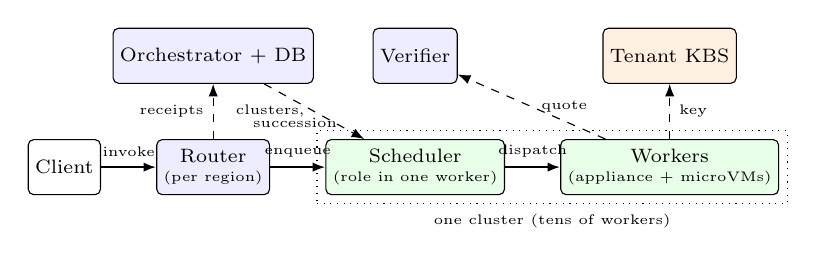
\begin{tikzpicture}[
  node distance=5mm and 7mm,
  box/.style={draw, rounded corners=2pt, minimum height=7mm, align=center, font=\scriptsize, inner sep=2.5pt},
  trusted/.style={box, fill=blue!7},
  attested/.style={box, fill=green!9},
  tenant/.style={box, fill=orange!12},
  arr/.style={-{Latex[length=1.6mm]}, thick},
  dsh/.style={-{Latex[length=1.6mm]}, dashed}]
  \node[box] (client) {Client};
  \node[trusted, right=of client] (router) {Router\\[-1pt]\tiny(per region)};
  \node[attested, right=of router] (sched) {Scheduler\\[-1pt]\tiny(role in one worker)};
  \node[attested, right=of sched] (worker) {Workers\\[-1pt]\tiny(appliance + microVMs)};
  \node[trusted, above=7mm of router] (orch) {Orchestrator + DB};
  \node[trusted, above=7mm of sched] (ver) {Verifier};
  \node[tenant, above=7mm of worker] (kbs) {Tenant KBS};
  \draw[arr] (client) -- node[above,font=\tiny]{invoke} (router);
  \draw[arr] (router) -- node[above,font=\tiny]{enqueue} (sched);
  \draw[arr] (sched) -- node[above,font=\tiny]{dispatch} (worker);
  \draw[dsh] (orch) -- node[left,font=\tiny]{clusters,} node[right,font=\tiny, xshift=-9mm, yshift=-1.5mm]{succession} (sched);
  \draw[dsh] (worker) -- node[right,font=\tiny]{quote} (ver);
  \draw[dsh] (worker) -- node[right,font=\tiny]{key} (kbs);
  \draw[dsh] (router) -- node[left,font=\tiny]{receipts} (orch);
  \node[draw, dotted, fit=(sched)(worker), inner sep=3pt, label={[font=\tiny]below:one cluster (tens of workers)}] {};
\end{tikzpicture}}
\caption{Roles. Blue: provider-run orchestrator tier (trusted for availability and accounting only). Green:
volunteer machines running the attested appliance (their \emph{hosts} may still omit or delay). Orange: tenant-operated
key broker. Solid arrows: the invocation path; dashed: control and trust.}
\label{fig:arch}
\end{figure}

\subsection{Donation sessions and attestation}
A worker alternates between \textsc{off} and \emph{sessions}. A session starts when the owner reboots into the
appliance (scheduled, idle-triggered, or on a dedicated spare box), becomes schedulable when attestation completes, and
ends abruptly (owner reboot, power loss) or gracefully (a drain request with a deadline). Session lengths are heavy-tailed
and time-of-day dependent, with regional shocks. The appliance image is a signed unified kernel image with a dm-verity
root, no owner login, and a data partition sealed to the expected PCR values; the disk caches survive a session as
ciphertext.

Attestation follows the Keylime pattern \cite{schear2016keylime}. The agent presents the TPM's endorsement-key
certificate, then a quote over PCRs and the IMA log bound to a nonce and a freshly generated session public key; the
verifier replays the event log against a policy and returns a session certificate that expires unless re-quoted. All
channels use mutual TLS under that certificate, so no untrusted OS lies on any path. A tenant's KBS releases that tenant's
key, wrapped to the session key, only to such a host. \emph{Trust-warm} means that the key is present in appliance memory
this session; it is lost with the session. The scheduler and orchestrator never see tenant keys.

\subsection{Threat model}
\label{sec:threat}
\emph{Volunteer owners} control power, network, firmware settings and their own OS, may try to boot modified software,
run the appliance in a VM, replay, delay or drop traffic, create identities, and choose when to defect. Measured boot, a
vendor-certified TPM endorsement key, an owner-locked image and sealed storage defeat the first group; what remains is
\emph{omission and timing}: power off, drop, delay, throttle, and lying about anything outside the attested stack
(including fake drain notices). \emph{Network attackers} see only ciphertext. \emph{Other tenants} are contained by
microVM isolation. Out of scope: lab-grade physical attacks (for example fTPM voltage glitching \cite{jacob2023faultpm}),
kernel and VMM zero-days in the appliance, side channels and traffic analysis, and failure of or attacks on the
orchestrator tier. Identity is the hash of the TPM endorsement key, so identities cost machines \cite{douceur2002sybil}.

\textbf{Consequence.} To the rest of the system a malicious worker or scheduler host is an omission/timing-faulty node.
The same mechanisms therefore cover churn, crashes and malice (Sec.~\ref{sec:design}).

\subsection{Substrate profiles}
\label{sec:substrates}
A \emph{substrate profile} is data that tells one generic lifecycle engine how a worker establishes trust, how long it
lasts, what the warm-state ladder looks like, and what assurance a host of that class carries. We model five.
\texttt{appliance\_tpm} (primary) pays a reboot, measured boot and a TPM quote once per session. \texttt{cvm\_snp}
and \texttt{coco\_pool} model server confidential VMs and confidential containers with per-wCVM or per-shell establishment and
trustlet-style warm levels, with parameters from the literature (ranges swept in experiments). \texttt{drtm\_hv} models
a measured hypervisor launched under the owner's OS (no reboot, owner interference). \texttt{none} is the unattested reference.

For appliance and unattested hosts the ladder has five levels per (worker, function): L0 nothing cached; L1 code bundle and
root file system on disk; L2 snapshot on disk; L3 warm idle VM in RAM; L4 busy. Trust is an orthogonal flag $K[t,j]$.

\subsection{Exposure}
Let $a_j\in[0,1]$ be the assurance of host $j$ (substrate base, freshness of the last quote, firmware policy), and
$\mathrm{KH}(t)$ the set of hosts holding tenant $t$'s key or decrypted artifacts. The \emph{exposure} of $t$ is
$E_t=\sum_{j\in \mathrm{KH}(t)}(1-a_j)$, weighted by the tenant's sensitivity class $\sigma_t$ in the planner. It is a
transparent proxy for the attack surface, not a probability of compromise, and we therefore report latency, exposure and
robustness side by side rather than as one weighted number.

\section{The \voss{} Design}
\label{sec:design}

\subsection{Why two timescales}
Trust and warm state are set-valued and long-lived: a key released to a host stays for the session; exposure depends on
\emph{how many distinct hosts} hold a key; and robustness to $f$ defectors is a worst case over subsets. None of these is a
per-assignment additive cost, so none belongs in a per-request optimization. Placement, in contrast, is latency-critical and
decomposes well. \voss{} therefore splits the decision (Fig.~\ref{fig:loops}): a \emph{slow loop} (the trust and warm-state
planner, every 10--60\,s and on events) decides which hosts are trust-warm for which tenants, which snapshots and warm VMs
to keep, and how many slots to earmark; a \emph{fast loop} places each invocation using that plan.

\begin{figure}[t]
\centering
\resizebox{\columnwidth}{!}{%
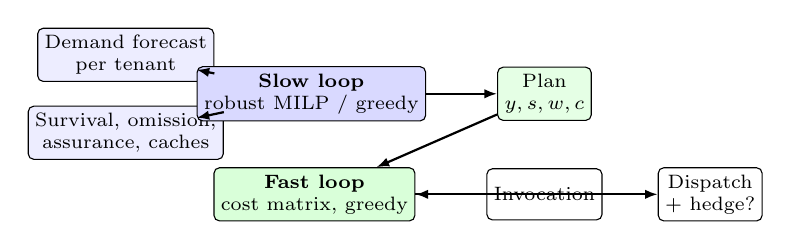
\begin{tikzpicture}[
  box/.style={draw, rounded corners=2pt, minimum height=6.5mm, align=center, font=\scriptsize, inner sep=2.5pt},
  arr/.style={-{Latex[length=1.6mm]}, thick}]
  \node[box, fill=blue!7] (fc) {Demand forecast\\per tenant};
  \node[box, fill=blue!7, below=3mm of fc] (hs) {Survival, omission,\\assurance, caches};
  \node[box, fill=blue!15, right=9mm of $(fc)!0.5!(hs)$] (plan) {\textbf{Slow loop}\\robust MILP / greedy};
  \node[box, fill=green!10, right=9mm of plan] (p) {Plan\\$y,s,w,c$};
  \node[box, below=6mm of p] (inv) {Invocation};
  \node[box, fill=green!15, left=9mm of inv] (fast) {\textbf{Fast loop}\\cost matrix, greedy};
  \node[box, right=7mm of inv] (disp) {Dispatch\\+ hedge?};
  \draw[arr] (fc) -- (plan); \draw[arr] (hs) -- (plan); \draw[arr] (plan) -- (p);
  \draw[arr] (p) -- (fast); \draw[arr] (inv) -- (fast); \draw[arr] (fast) -- (disp);
\end{tikzpicture}}
\caption{Two timescales. The planner decides where trust and warm state live; the placer decides where each
invocation runs, over candidates and earmarks the plan provides.}
\label{fig:loops}
\end{figure}

\subsection{Slow loop: trust and warm-state planning}
\label{sec:planner}
For one cluster with attested workers $J$ and \emph{hot} tenants and functions (those above a rate threshold; the long
tail uses a cold path), the planner chooses
$y[t,j]\in\{0,1\}$ (tenant $t$ is trust-warm on $j$), $s[f,j]\in\{0,1\}$ (snapshot of $f$ pinned on $j$),
$w[f,j]\in\mathbb{Z}_{\ge0}$ (warm VMs of $f$ on $j$), and $c[t,j]\ge0$ (slots of $j$ earmarked for $t$).
Inputs are estimates only: slots $\mathrm{cap}_j$, the survival probability $S_j(H)$ over the horizon, the omission rate
$p_j$, assurance $a_j$, failure domain $d(j)$, the demand quantile $q_t$ (a Poisson quantile of the forecast arrival
rate times service time), sensitivity $\sigma_t$, assurance floor $a_{\min,t}$ and robustness level $f_t$. The objective
(minimized; terms are logged separately) is
\begin{align}
\min\;&\sum_t C_t u_t + \sum_j\Big(\rho_{\mathrm{mem}}\sum_f m_f w[f,j]+\rho_{\mathrm{ssd}}\sum_f z_f s[f,j]\Big)\nonumber\\
&+\sum_{t,j}\sigma_t(1-a_j)\,y[t,j]+\kappa\!\sum_{t,j}(y[t,j]-y^{\mathrm{prev}}[t,j])^{+}\nonumber\\
&-\sum_{f,j}\beta\,b_f\,(w[f,j]+\gamma s[f,j]),
\label{eq:obj}
\end{align}
that is: uncovered demand $u_t$ priced at the cold penalty $C_t$, donor memory and storage, exposure, plan churn, and the
start-up time saved by warm VMs and snapshots (memory $m_f$, snapshot size $z_f$, benefit $b_f$). The central constraint is
robust coverage: with at most $f_t$ of the earmarked hosts defecting,
\begin{align}
&\sum_j c[t,j]\,S_j(H)(1-p_j)\;-\;\big(f_t\,\theta_t+\textstyle\sum_j \pi[t,j]\big)+u_t\;\ge\;q_t,\nonumber\\
&\pi[t,j]\ge c[t,j]-\theta_t,\quad \pi[t,j]\ge0,
\label{eq:robust}
\end{align}
where $f_t\theta_t+\sum_j\pi[t,j]$ equals the sum of the $f_t$ largest contributions by LP duality, the construction of
\cite{bertsimas2004price}. Because the constraint holds against \emph{any} $f_t$ hosts, including ones with a perfect
record, robustness does not depend on the omission model. Further constraints couple the variables ($c\le\mathrm{cap}\,y$,
$w\le W_{\max}\,y$, $s\le y$), bound slots, memory and SSD per host, cap the share of earmarked capacity in any failure
domain by $\kappa_{\mathrm{dom}}$, forbid $y[t,j]=1$ when $a_j<a_{\min,t}$ or the attestation expires within the horizon,
and the default $f_t=\lceil\alpha_{\mathrm{assumed}}N_{\mathrm{cluster}}\rceil$. A cluster has about 30 workers, at most 20
hot tenants and 50 hot functions, so the program has $10^3$--$3\cdot10^3$ integers; we solve it with HiGHS
\cite{huangfu2018highs} within a time limit and fall back to the incumbent and then to a greedy planner that adds workers by
value density until the robust coverage holds. The plan is diffed against its predecessor into idempotent actions
(\textsc{prepare}, \textsc{pin-snapshot}, \textsc{warm}, \textsc{release}), rate-limited per worker; the fast loop only
relies on state workers have \emph{confirmed}.

\subsection{Fast loop: placement, hedging and routing}
For an invocation of tenant $t$, candidates are the confirmed trust-warm workers (with earmarked slots) and, behind them,
other attested workers meeting the assurance floor, which pay a key-release round trip and an exposure increment. Each
pair $(i,j)$ gets a completion distribution (a moment-matched shifted lognormal over wait, trust, start-up by ladder
level, network and execution) and a failure probability $p_{\mathrm{fail}}=1-S_j(T)(1-p_j)$. The default scalarization is
$w_i\,p_{\mathrm{miss}}+\epsilon\,\mathbb{E}[T]+\lambda_{\mathrm{exp}}\,\mathrm{exposure}$. Execution time comes from a
Bayesian log-linear predictor with hierarchical shrinkage and conformal calibration \cite{shafer2008conformal}. If
$p_{\mathrm{miss}}$ of the best candidate exceeds a threshold $\theta$ and a per-cluster budget allows, \voss{} sends a
\emph{tied} duplicate to the best trust-warm candidate in a \emph{different failure domain} and cancels the loser on the
first result \cite{dean2013tail}; attested results make duplicates integrity-safe. Routers pick the cluster with a score
$\mathrm{rtt}+\mathbb{E}[\mathrm{completion}]+\mathrm{health}+\mathrm{trust\_cold\_penalty}$, so spilling to a cluster
without trust-warm capacity is a priced decision.

\subsection{Fault tolerance: liveness is a hint, progress is evidence}
\label{sec:ft}
A black-holing owner keeps heartbeating, so heartbeats cannot be evidence. \voss{} detects \emph{progress}: routers (trusted)
time \textsc{enqueue} without \textsc{accepted}; schedulers time \textsc{accepted} without \textsc{result} at the predicted
completion quantile; the orchestrator watches the scheduler's attested placement latency; and a CUSUM change-point test
over outcomes defeats on-off defection. A suspect worker loses new work and trust-warm eligibility and its in-flight work
is hedged or retried; fake drain notices only make the scheduler more conservative and never excuse an omission.

\emph{Succession without consensus.} Because the orchestrator is a reliable arbiter, a failed scheduler is replaced by an atomic
compare-and-swap on the cluster epoch in the operational database; the appointment token binds the cluster, epoch and the
\emph{session-certificate} of the successor, so a cloned image is not appointed, and workers fence lower epochs.
Schedulers keep only soft state: undispatched invocations live in the router, running work in the workers (recovered by a
roll call), and plan and learned state in a checkpoint. A restarted or rolled-back appliance is a new instance and must be
re-appointed, which closes the rollback caveat of trusted-hardware protocols.

\subsection{Receipts and credits}
Each result carries a receipt signed by the worker's session key (invocation, attempt, worker, certificate, epoch, execution
time, reference work units, output digest). A host cannot claim work it did not do, only fail to do work. Credits are paid
in \emph{reference work units}, not elapsed time, so throttling earns nothing; donor caching earns a small credit only while
the worker answers probes. Reputation, an identity-level long-run signal, feeds rewards and planner tie-breaks but never the
failure probability $p_{\mathrm{fail}}$, which is fed separately by session survival and omission, to avoid double counting.

\section{How We Evaluate}
\label{sec:method}

A volunteer platform with thousands of machines, controlled churn, hostile owners and paired comparisons of policies cannot be run on real hardware. We evaluate \voss{} in a deterministic simulator and calibrate it against measurements. This section says what the simulator models, where its numbers come from, how far we checked it, and how every comparison is made.

\subsection{The simulator}
\label{sec:sim}
The simulator is a single-threaded discrete-event simulator in Python. Simulated time jumps from one event to the next in a fixed order, and every random draw comes from a named, seeded stream, so a run can be repeated exactly.
A run takes a configuration, a calibration bundle and a seed. It first draws everything the system under test cannot influence: the machines, every session start and end, which owners are adversaries, the arrivals and the noise in each execution. These traces are content-hashed, so two systems compared on one seed face the same world.
The engine then runs the actors (workers, schedulers, routers, orchestrator, verifier, key services) and the policies. Policies see only immutable views built from messages, never the world itself. At the end, checks assert that every success ran on an attested host after a key release, that each invocation has one outcome, and that the time components add up to the measured latency. Analysis reads only the raw tables.

\textbf{Nothing is free.} Every interaction is a message that arrives after a delay from the distance between about 100 cities (100\,km per millisecond, times 1.3 for route detours), plus last-mile delay and jitter. Disk reads, CPU contention, TPM quotes, key release and the decision time of planner, placer, router and orchestrator all consume simulated time.
Decision time is a fixed part plus a part proportional to the work, so results do not depend on the speed of the machine running the simulation. The coefficients are placeholders from the literature, not measurements. For the planner the charge is about 0.1\,s, for the greedy and the exact planner alike, while the exact planner really takes \MilpSolveS\,s, so its results are optimistic about how stale its plans are.

\textbf{The world.} Workers come in three tiers (nightly, idle-hours, dedicated) with different hardware, cities and trust substrates. Session lengths are heavy-tailed with time-of-day effects, most departures are abrupt, and correlated shocks remove a share of a city at once.
No public trace of consumer donation sessions exists, so we follow volunteer-availability studies~\cite{javadi2013fta}, mark the parameters \emph{assumed} and sweep them. The workload has six tenants and 12 functions modelled on SeBS~\cite{copik2021sebs}, in three service classes, with skewed popularity and bursty, day-and-night arrivals~\cite{shahrad2020wild}. 11 of the 12 functions are marked idempotent, by our assumption.
A fraction $\alpha$ of workers are adversaries who omit, delay, black-hole, defect after building a record, send fake drain notices, or collude within a failure domain. By Property 1 none of them forges results or reads keys on an attested substrate, while the unattested reference allows both.

\subsection{Calibration and what we checked}
\label{sec:calib}
Parameters from the specification are literature values or assumptions and are tagged so. Measured values come only from calibration bundles. We measured one on a consumer laptop (\CalCpu, a discrete TPM~2.0, a hard disk), which stands in for a donor machine.
A harness reboots it into the appliance and records timestamps at about one-second resolution, and microbenchmarks cover TPM quotes, hashing, microVM boot and snapshots. Compared with our placeholders, reboot to kernel is slower (\CalReboot\,s against \CalRebootPh\,s), the phase from kernel start to a running agent is far slower (\CalUserspace\,s), and creating a 512\,MB snapshot on a hard disk takes \CalSnapCreate\,s.
From power-on, an attested worker takes \CalAttested\,s (median of \CalAttestedN{} boots, \CalAttestedKernel\,s of it after kernel start). A warm-cache microVM boot takes \CalFcBootWarmMs\,ms, close to published figures~\cite{agache2020firecracker}.

Two limits apply. The laptop is not the intended donor machine and lacks AMD SEV-SNP and Intel TDX, so confidential-VM parameters are literature values, which we sweep~\cite{misono2025cvm,holmes2024severifast,li2023bifrost}.
And the appliance ran in \emph{host mode} (the measurement chain and quote on the host, microVMs through Firecracker) rather than as a locked image on bare metal. The attested-session figure is a measured sum, not a measured attestation of the final image.

\textbf{A first check against real execution (E01).} To test the start-up and execution parts of the simulator, we ran the same scenarios in a single-box emulation on a lab node (Intel Core i7-12700, 125\,GB, NVMe, Firecracker 1.10.1) and in the simulator, with a calibration measured on that node. The emulation uses real microVMs for boot, snapshot restore, dispatch and function execution, and keeps network, key release, attestation and queueing as models (16 donor slices, five functions, ten minutes per run, three seeds).
Success rate agrees within 0.6 percentage points in every scenario, the mix of start-up levels is identical, and median synchronous latency agrees within 6--23\%. The \emph{shape} of the latency distribution does not meet our pre-set cut-offs, so every scenario is graded ``partly'' close and none ``close''. At light load the simulator's P99 is 3.7 to 4.1 times the emulation's, driven by a handful of cold invocations: the P99 of about 530 requests is the five slowest.
E01 does not test the network, attestation, key release, session boot or failure detection at scale, and no multi-machine deployment has validated the simulator end to end. We therefore read differences between designs, not absolute latencies.

\subsection{Protocol}
\label{sec:protocol}
Each experiment is a frozen specification, and every cell is run with ten seeds (three for the two largest scalability points). Unless stated, \voss{} uses the greedy planner and the default placer, router and hedger. Systems in a comparison share the world and the per-invocation random draws, so each comparison is \emph{paired} by seed.
For a metric we take the per-seed difference and report its mean with a 95\% bootstrap interval~\cite{efron1993bootstrap}. Percentiles are computed per run, then averaged, never pooled.

Each hypothesis is written down before the run with a mechanical rule. It is \emph{supported} if the interval excludes zero in the predicted direction by at least a stated margin, \emph{weak} if it excludes zero but the effect is below the margin, \emph{inconclusive} if the interval includes zero, and \emph{refuted} if it excludes zero the other way.
The manuscript's numbers and tables are generated from the result tables by a script that also fails if a result stops supporting the sentence it backs.

We report success, the share of deadlines met, median and P99 synchronous latency, \emph{waste} (extra attempts per success), donor memory held warm, and key exposure. A system is \emph{feasible} in a scenario cell if the lower 95\% bound of its success is at least 0.99 and either its deadline-met share or its P99 meets a target.
Feasibility maps then show \emph{where} each design works, rather than an average.

\textbf{Baselines} run on the same simulator, candidates and cost model and differ only in the registered policy: no planning (provision on arrival), keep-alive with a time limit, a heartbeat-only detector, and $f=0$ (no robustness). The \emph{simple baseline} combines static regional clusters, nearest-region routing, least-loaded placement, keep-alive and no hedging.
Commercial-style references (\emph{Lambda-like}, \emph{Azure-like}) are always-on datacenter hosts with per-function keep-alive and nearest-region routing, priced from list prices, on the same engine.

\subsection{Reproducibility}
\label{sec:repro}
Every number, table and figure in Section~\ref{sec:results} is regenerated from raw run logs by committed scripts, and runs are bit-reproducible: re-executing a run gives raw tables with the same result hash, recorded in a manifest with the scenario and calibration hashes. Floating-point arithmetic repeats bit for bit only under stated conditions, because a last-bit difference can flip a near-tie in placement and send the whole trajectory elsewhere.
We found that NumPy's maths functions use different code paths on CPUs with and without AVX-512, and a first verification re-run failed for exactly this reason. We now pin NumPy to the SSE4 baseline that every x86-64 CPU supports and record a canary hash of the maths functions in each manifest.
The full sweep, 21 experiments and 2{,}366 runs, was then re-executed on independently provisioned machines, and 2{,}366 of 2{,}366 hashes matched.
Reproduction needs an x86-64 CPU with fused multiply-add, Linux with glibc, Python 3.11 and the committed lockfile, and about four hours of wall-clock time as parallel jobs. No TPM or special hardware is needed. Appendix~\ref{app:repro} gives the requirements, checks and commands.

\section{Results}
\label{sec:results}

Unless stated, differences are paired by seed over 10 seeds with 95\% bootstrap intervals; the complete list of
hypotheses and verdicts is Table~\ref{tab:score}. Where a result contradicts a design claim we say so in the section where it appears.

\subsection{Trust establishment and cold start (E-CS1)}
\label{sec:res-cs1}
Table~\ref{tab:cs1} gives, per substrate, the simulated time to establish a donation session and the start latency from each
level of the warm-state ladder. Two facts shape everything that follows. First, the appliance pays a large \emph{one-off}
cost per session (\SimApplSession\,s with the pre-measurement parameters; \CalAttested\,s measured end to end on the
laptop), against \SimCvmSession\,s for a confidential VM and \SimCocoSession\,s for a confidential-container pool: trust on the appliance
is expensive to establish and everything is lost when the session ends. Second, once the session exists the appliance is as fast as
an unattested Firecracker host: warm and snapshot starts are within a few percent of the unattested figures (H5, supported), because
attestation is paid per session rather than per invocation. Confidential VMs invert the trade: cheap sessions but slower
lower ladder levels (Table~\ref{tab:cs1}). Our
a-priori expectation that confidential-VM classes establish trust 10--100$\times$ \emph{slower} than the appliance is refuted:
they are about 93\% faster, because the appliance's cost is a reboot. Measurements on the laptop agree with the simulated
ladder: a warm Firecracker start takes \CalFcBootWarmMs\,ms, a cold-cache boot \CalFcBootColdS\,s, and creating a 512\,MB
snapshot \CalSnapCreate\,s on a hard disk, which makes snapshots something to plan rather than to take on demand.

\begin{table}[t]
\caption{Simulated session establishment and start latency (s) from each warm-state level (L0 nothing cached, L3 warm idle
VM; ``--'' not applicable). Pre-measurement parameters (Table~\ref{tab:calib}).}
\label{tab:cs1}
\centering\scriptsize
\resizebox{\columnwidth}{!}{% Generated by experiments/paper_tex.py; do not edit.
\begin{tabular}{lrrrrr}
\toprule
\textbf{Substrate} & \textbf{Session} & \textbf{L0} & \textbf{L1} & \textbf{L2} & \textbf{L3} \\
\midrule

appliance (TPM) & 19.2 & 1.45 & 0.346 & 0.0285 & 0.00197 \\
DRTM hypervisor & 2.31 & 1.44 & 0.34 & 0.0284 & 0.00196 \\
CVM (SEV-SNP) & 1.41 & 2.31 & 1.19 & 0.155 & 0.002 \\
CoCo pool & 8.11 & 2.25 & 1.14 & -- & 0.002 \\
no attestation & 1.06 & 1.45 & 0.344 & 0.0278 & 0.00201 \\
\bottomrule
\end{tabular}
}
\end{table}

\subsection{Where is the system viable? (E20)}
\label{sec:res-viab}
Averages hide the regimes in which a design fails, so we map viability (Sec.~\ref{sec:method}) over three two-dimensional
panels. Figure~\ref{fig:viab} colors each cell by which system is viable under the default criterion (success $\ge0.99$ and deadline-met $\ge0.95$) and prints \voss{}'s P99.
Table~\ref{tab:viab} counts \voss{}-viable cells under other targets.

\begin{figure*}[t]
\centering
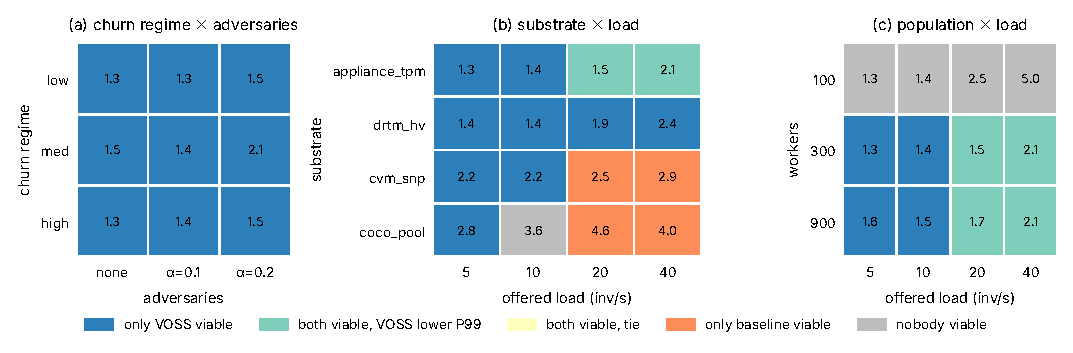
\includegraphics[width=\textwidth]{figures/fig_viability}
\caption{Viability maps (E20). Cell color: which of \voss{} and the best simple baseline is viable (success $\ge0.99$,
deadline-met $\ge0.95$); numbers: \voss{} sync P99 in seconds. (a) churn regime against adversary fraction, (b) substrate against offered load (inv/s),
(c) population against offered load.}
\label{fig:viab}
\end{figure*}

\begin{table}[t]
\caption{Number of cells in which \voss{} is viable, by target (deadline-met fraction, or absolute sync P99).}
\label{tab:viab}
\centering\scriptsize
\resizebox{\columnwidth}{!}{% Generated by experiments/paper_tex.py; do not edit.
\begin{tabular}{lrrrrrrr}
\toprule
\textbf{Panel} & \textbf{0.90} & \textbf{0.95} & \textbf{0.98} & \textbf{2 s} & \textbf{3 s} & \textbf{5 s} & \textbf{Cells} \\
\midrule
& \multicolumn{3}{c}{deadline-met target} & \multicolumn{3}{c}{sync P99 target} & \\
\cmidrule(lr){2-4}\cmidrule(lr){5-7}
A: churn $\times$ $\alpha$ & 9 & 9 & 0 & 8 & 9 & 9 & 9 \\
B: substrate $\times$ load & 16 & 11 & 0 & 6 & 13 & 16 & 16 \\
C: $N$ $\times$ load & 8 & 8 & 0 & 8 & 10 & 10 & 12 \\
\bottomrule
\end{tabular}
}
\end{table}

\voss{} is the \emph{only} viable system in all \ViabACells{} cells of panel A, which spans three churn regimes and up to $20\%$ omitting owners, in
\ViabBMetOnly{} of \ViabBCells{} cells of panel B and in \ViabCMetOnly{} of \ViabCCells{} cells of panel C. With an absolute sync P99 target of 3\,s
it is viable in \ViabAPThreeVoss{} of \ViabACells, \ViabBPThreeVoss{} of \ViabBCells{} and \ViabCPThreeVoss{} of \ViabCCells{} cells, and the simple baseline in none of them; at
5\,s \voss{} is viable in \ViabAPFiveVoss, \ViabBPFiveVoss{} and \ViabCPFiveVoss{} cells. The two criteria measure different things (a deadline is a multiple of the
warm latency; the absolute target is what a user perceives), which is why a baseline can pass one and fail the other.

The map also shows where \voss{} is \emph{not} the right choice. On confidential-VM and confidential-container substrates at higher load, the simple baseline
is the only viable system in \ViabBMetBase{} cells (Fig.~\ref{fig:viab}b): we conjecture that with cheap session establishment there is little cold-start cost for planning to remove, while it still adds exposure and memory;
we did not test this. With 100 workers no system is viable in any cell of panel C
(\ViabCMetNoneFive{} cells), so the design needs a minimum population, and at a deadline-met target of 0.98 \emph{no} system is viable in any cell: the
``98\% of sync invocations within $5\times$ warm latency'' service level is out of reach in this setting for \voss{} and the baselines alike.

\subsection{Planning trust and warm state (E04, E19)}
\label{sec:res-plan}
Table~\ref{tab:plan} compares planners on the same scenarios under medium and high churn. Planning is the largest single lever: the robust MILP
cuts sync P99 by \HOnePctNoneMed\% (medium churn) and \HOnePctNoneHigh\% (high churn) against no planning, and by \HOnePctKeepMed\% and
\HOnePctKeepHigh\% against a keep-alive TTL (H1, supported). It pays with donor memory: about \MilpWarmRatio$\times$ the warm memory of
keep-alive at medium churn. The comparison that
motivates the integer program is weaker. The MILP is only \HEightPct\% better than the greedy planner at high churn (H8, interval includes
zero, inconclusive) while its solve time is \MilpSolveS\,s per cluster against \GreedySolveMs\,ms. We cannot, on this evidence, claim that the
exact solver pays for itself. What it gives, beyond latency, is the coverage guarantee of Eq.~\eqref{eq:robust}, whose value is shown below.

\begin{table}[t]
\caption{Planner comparison (E04): mean $\pm$ 95\% half-width over 10 seeds. Met: deadline-met fraction; Warm: GB of idle warm memory.}
\label{tab:plan}
\centering\scriptsize
\resizebox{\columnwidth}{!}{% Generated by experiments/paper_tex.py; do not edit.
\begin{tabular}{llrrrrr}
\toprule
\textbf{Regime} & \textbf{Planner} & \textbf{P99 (s)} & \textbf{Met} & \textbf{Warm GB} & \textbf{Exposure} & \textbf{Solve (s)} \\
\midrule

churn\_med & no planning & 2.78{\scriptsize$\pm$1.35} & 0.940{\scriptsize$\pm$0.017} & 1{\scriptsize$\pm$0} & 8.5{\scriptsize$\pm$1.4} & 0.001{\scriptsize$\pm$0.000} \\
churn\_med & keep-alive TTL & 1.78{\scriptsize$\pm$0.48} & 0.971{\scriptsize$\pm$0.018} & 61{\scriptsize$\pm$9} & 7.4{\scriptsize$\pm$1.1} & 0.002{\scriptsize$\pm$0.001} \\
churn\_med & greedy planner & 1.29{\scriptsize$\pm$0.09} & 0.978{\scriptsize$\pm$0.015} & 94{\scriptsize$\pm$14} & 19.9{\scriptsize$\pm$1.8} & 0.005{\scriptsize$\pm$0.000} \\
churn\_med & robust MILP & 1.26{\scriptsize$\pm$0.11} & 0.979{\scriptsize$\pm$0.014} & 131{\scriptsize$\pm$19} & 20.1{\scriptsize$\pm$1.7} & 3.333{\scriptsize$\pm$0.457} \\
churn\_high & no planning & 3.48{\scriptsize$\pm$1.32} & 0.923{\scriptsize$\pm$0.029} & 1{\scriptsize$\pm$0} & 7.5{\scriptsize$\pm$1.2} & 0.001{\scriptsize$\pm$0.000} \\
churn\_high & keep-alive TTL & 3.28{\scriptsize$\pm$1.91} & 0.940{\scriptsize$\pm$0.030} & 59{\scriptsize$\pm$10} & 7.3{\scriptsize$\pm$0.9} & 0.001{\scriptsize$\pm$0.000} \\
churn\_high & greedy planner & 1.42{\scriptsize$\pm$0.17} & 0.958{\scriptsize$\pm$0.028} & 87{\scriptsize$\pm$13} & 15.8{\scriptsize$\pm$1.2} & 0.006{\scriptsize$\pm$0.001} \\
churn\_high & robust MILP & 1.38{\scriptsize$\pm$0.16} & 0.959{\scriptsize$\pm$0.031} & 115{\scriptsize$\pm$12} & 15.0{\scriptsize$\pm$0.8} & 3.291{\scriptsize$\pm$0.502} \\
\bottomrule
\end{tabular}
}
\end{table}

Figure~\ref{fig:abl} removes one component of \voss{} at a time (E19). Removing lifecycle-aware placement costs
\AblLifecycleP\,s of sync P99, removing planning \AblPlanningP\,s (and lowers exposure by \AblPlanningExp, because less is pre-warmed and fewer hosts hold keys), removing the robust
constraint \AblRobustP\,s (exposure \AblRobustExp{} lower) and removing hedging \AblHedgeP\,s. Geo-clustering is the only component whose removal
\emph{improves} P99 (\AblGeoP\,s lower), and it also cuts exposure by \AblGeoExp: Sec.~\ref{sec:res-geo}. Putting reputation into the cost matrix instead of using it
as a tie-breaker raises exposure by \AblRepExp. The ablations also show where trust and latency trade against each other: the same components that buy P99
(planning, robustness) raise exposure.

\begin{figure}[t]
\centering
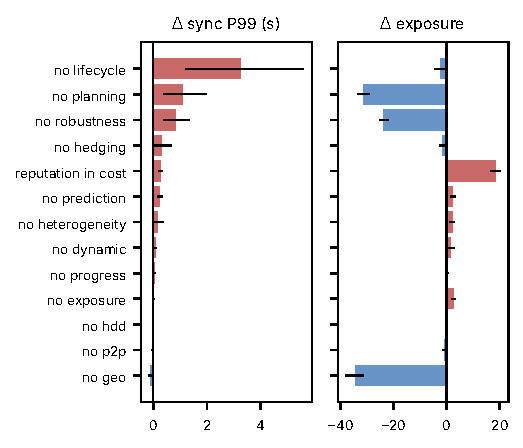
\includegraphics[width=\columnwidth]{figures/fig_ablation}
\caption{Ablations (E19): change when a component is removed, relative to full \voss{} (paired, 95\% intervals).
Left: sync P99; right: key-holder exposure.}
\label{fig:abl}
\end{figure}

\subsection{Faults, adversaries and the latency--exposure trade-off (E08, E15, E16, E23)}
\label{sec:res-ft}

\medskip\noindent\textbf{Detection.}
Table~\ref{tab:faults} injects crashes, partitions, black-holing and slowed scheduler hosts. Heartbeats alone cannot see a black hole: the
host keeps sending liveness while dropping work, so detection waits for the 60\,s timeout (\BhDetectHb\,s) and the run suffers \BhTimeoutsHb{} timeouts, against
\BhDetectProg\,s and \BhTimeoutsProg{} with progress-based detection (H-FT1, supported). For plain crashes progress detection needs \CrashDetectProg\,s and
failover \CrashFailover\,s. A slowed-but-live scheduler is the hardest case: failover takes \SlowFailover\,s on average because progress evidence must
accumulate before the slowdown is distinguishable from load.

\begin{table}[t]
\caption{Scheduler faults (E15): time to detection, failover, success and P99 within the fault window.}
\label{tab:faults}
\centering\scriptsize
\resizebox{\columnwidth}{!}{% Generated by experiments/paper_tex.py; do not edit.
\begin{tabular}{llrrrr}
\toprule
\textbf{Fault} & \textbf{Detector} & \textbf{Detect (s)} & \textbf{Failover (s)} & \textbf{Success (\%)} & \textbf{P99 in window (s)} \\
\midrule

crash & progress & 2.2{\scriptsize$\pm$0.3} & 2.7{\scriptsize$\pm$0.4} & 99.95{\scriptsize$\pm$0.02} & 1.28{\scriptsize$\pm$0.15} \\
crash & heartbeat\_only & 5.0{\scriptsize$\pm$0.0} & 5.5{\scriptsize$\pm$0.5} & 99.87{\scriptsize$\pm$0.04} & 1.66{\scriptsize$\pm$0.33} \\
partition & progress & 2.2{\scriptsize$\pm$0.3} & 2.6{\scriptsize$\pm$0.4} & 99.95{\scriptsize$\pm$0.02} & 1.28{\scriptsize$\pm$0.16} \\
partition & heartbeat\_only & 5.0{\scriptsize$\pm$0.0} & 5.5{\scriptsize$\pm$0.5} & 99.87{\scriptsize$\pm$0.04} & 1.67{\scriptsize$\pm$0.31} \\
blackhole & progress & 4.2{\scriptsize$\pm$3.0} & 4.6{\scriptsize$\pm$3.0} & 99.95{\scriptsize$\pm$0.02} & 1.28{\scriptsize$\pm$0.15} \\
blackhole & heartbeat\_only & 60.0{\scriptsize$\pm$0.0} & 59.3{\scriptsize$\pm$1.1} & 96.81{\scriptsize$\pm$0.51} & 2.90{\scriptsize$\pm$0.08} \\
slow & progress & 13.9{\scriptsize$\pm$7.9} & 14.3{\scriptsize$\pm$8.2} & 99.95{\scriptsize$\pm$0.03} & 1.34{\scriptsize$\pm$0.14} \\
slow & heartbeat\_only & 60.0{\scriptsize$\pm$0.0} & 59.3{\scriptsize$\pm$1.1} & 99.55{\scriptsize$\pm$0.41} & 2.00{\scriptsize$\pm$0.33} \\
\bottomrule
\end{tabular}
}
\end{table}

\medskip\noindent\textbf{Omitting owners.}
Table~\ref{tab:adv} sweeps the fraction $\alpha$ of omitting owners. With $\alpha=0.2$ \voss{} keeps success at \VossSuccAlpha\%, whereas
heartbeat-only detection with otherwise identical machinery drops to \HbSuccAlpha\% (H4, supported). Progress detection also gives
\HbOmitRatio$\times$ fewer results dropped by omitting owners at $\alpha=0.2$. The hypothesis that the \emph{robust} planning constraint is what keeps success
is not supported: setting $f=0$ changes success by only \FzeroSuccDelta{} percentage points (H2, inconclusive), though it lengthens P99 (Table~\ref{tab:adv}).
Detection and re-dispatch, not redundant coverage, carry the success; robust planning buys tail latency.

\begin{table}[t]
\caption{Omitting owners (E08), mean $\pm$ 95\% half-width over 10 seeds. Omissions: results dropped by adversaries.}
\label{tab:adv}
\centering\scriptsize
\resizebox{\columnwidth}{!}{% Generated by experiments/paper_tex.py; do not edit.
\begin{tabular}{llrrrr}
\toprule
\textbf{Adversaries} & \textbf{System} & \textbf{Success (\%)} & \textbf{P99 (s)} & \textbf{Waste (\%)} & \textbf{Omissions} \\
\midrule

none $\alpha$=0 & VOSS & 99.99{\scriptsize$\pm$0.01} & 1.27{\scriptsize$\pm$0.11} & 1.7{\scriptsize$\pm$0.5} & 0{\scriptsize$\pm$0} \\
none $\alpha$=0 & VOSS, $f{=}0$ & 99.99{\scriptsize$\pm$0.01} & 1.60{\scriptsize$\pm$0.24} & 2.2{\scriptsize$\pm$0.6} & 0{\scriptsize$\pm$0} \\
none $\alpha$=0 & heartbeat-only & 99.98{\scriptsize$\pm$0.01} & 1.36{\scriptsize$\pm$0.15} & 2.0{\scriptsize$\pm$0.7} & 0{\scriptsize$\pm$0} \\
mixed $\alpha$=0.1 & VOSS & 99.95{\scriptsize$\pm$0.04} & 1.32{\scriptsize$\pm$0.12} & 2.2{\scriptsize$\pm$0.5} & 38{\scriptsize$\pm$14} \\
mixed $\alpha$=0.1 & VOSS, $f{=}0$ & 99.96{\scriptsize$\pm$0.03} & 2.15{\scriptsize$\pm$0.60} & 2.9{\scriptsize$\pm$0.6} & 37{\scriptsize$\pm$11} \\
mixed $\alpha$=0.1 & heartbeat-only & 98.19{\scriptsize$\pm$0.75} & 1.36{\scriptsize$\pm$0.13} & 4.0{\scriptsize$\pm$0.9} & 298{\scriptsize$\pm$115} \\
mixed $\alpha$=0.2 & VOSS & 99.95{\scriptsize$\pm$0.03} & 1.43{\scriptsize$\pm$0.16} & 2.6{\scriptsize$\pm$0.5} & 61{\scriptsize$\pm$13} \\
mixed $\alpha$=0.2 & VOSS, $f{=}0$ & 99.83{\scriptsize$\pm$0.17} & 2.05{\scriptsize$\pm$0.52} & 3.5{\scriptsize$\pm$0.8} & 80{\scriptsize$\pm$31} \\
mixed $\alpha$=0.2 & heartbeat-only & 96.79{\scriptsize$\pm$1.13} & 1.39{\scriptsize$\pm$0.16} & 5.6{\scriptsize$\pm$1.3} & 527{\scriptsize$\pm$161} \\
all $\alpha$=0.2 & VOSS & 99.94{\scriptsize$\pm$0.05} & 1.37{\scriptsize$\pm$0.10} & 2.3{\scriptsize$\pm$0.7} & 31{\scriptsize$\pm$9} \\
all $\alpha$=0.2 & VOSS, $f{=}0$ & 99.96{\scriptsize$\pm$0.03} & 2.28{\scriptsize$\pm$1.00} & 2.7{\scriptsize$\pm$0.5} & 28{\scriptsize$\pm$8} \\
all $\alpha$=0.2 & heartbeat-only & 97.70{\scriptsize$\pm$1.26} & 1.42{\scriptsize$\pm$0.14} & 5.2{\scriptsize$\pm$2.4} & 385{\scriptsize$\pm$227} \\
\bottomrule
\end{tabular}
}
\end{table}

\medskip\noindent\textbf{Hedging.}
Hedging duplicates risky invocations. Always hedging cuts P99 but wastes \AlwaysWastePct\% extra attempts. Risk-proportional hedging (hedge with probability
tied to estimated risk, within a 5\% budget) wastes \RpWastePct\%, and its P99 is \HedgePNinetyninePct\% lower with $\alpha=0.1$ but with an interval from
\HedgePNinetynineLo\% to $+$\HedgePNinetynineHi\% (H-FT3, inconclusive). It is cheap insurance, not demonstrated to be necessary.

\medskip\noindent\textbf{Pareto front.}
Robustness $f$ and the exposure weight trade latency against key-holder exposure (E23, Fig.~\ref{fig:pareto}). The aggregate front has \ParetoFrontN{}
points. Exposure grows with $f$ (\ExpFZero, \ExpFOne{} and \ExpFTwo{} at $f=0$, $0.1$, $0.2$), consistent with covering any $f$ failures requiring more key-holding hosts. Aggregate sync P99 stays
within \ParetoPNinetynineLo--\ParetoPNinetynineHi\,s across configurations, so the knee at $f=\ParetoKneeF$ saves \ParetoKneeExpSaved\% of exposure against the best-latency front point for
\ParetoKneePNinetynineLoss\% more P99 (H3, supported): moderate exposure budgets are cheap. Per tenant class the picture is less benign. Low-sensitivity tenants stay at about \ParetoLowMax\,s or below, but for
high-sensitivity tenants P99 reaches \ParetoHighMax\,s in one robust configuration, while an $f=0$ configuration has the lowest exposure at nearly the best P99. The aggregate knee therefore should not be applied to every class;
sensitivity classes need their own operating point.

\begin{figure}[t]
\centering
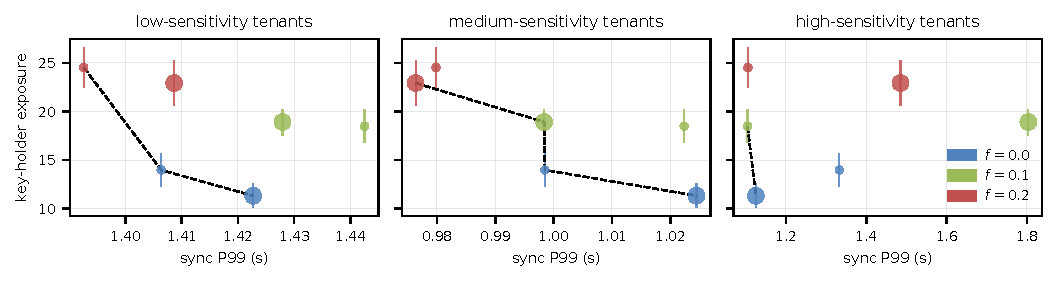
\includegraphics[width=\columnwidth]{figures/fig_pareto}
\caption{Latency--exposure--robustness (E23). Each point is a ($f$, exposure weight) configuration (marker size: weight) with 95\% error bars on exposure;
the dashed line is the Pareto front per tenant sensitivity class.}
\label{fig:pareto}
\end{figure}

\subsection{Geography, routing and caching (E05--E07, E09)}
\label{sec:res-geo}
The geographic hierarchy, a central idea of the design, does not pay off at the scale we simulate. Table~\ref{tab:geo} compares a single global scheduler
against static regions, static $k$-means and dynamic clusters. Dynamic clusters have \emph{higher} P99 than the global scheduler by
\HSevenEu\% (Europe), \HSevenEuNa\% (EU+NA) and \HSevenWorld\% (world) (H7, refuted at all three populations), and hold \GeoExpRatio$\times$ the key-holder
exposure in Europe, since each of the \GeoClusters{} clusters must cover demand with its own key holders. The network share of latency
does fall in some populations (Table~\ref{tab:geo}), but not enough to offset the cost of splitting the pool. We attribute this to fewer hosts per
cluster for pooling warm state and keys, but did not isolate the mechanism. Our results show no population in which geo-clustering wins at the scale we simulate.

\begin{table}[t]
\caption{Geo-clustering (E05): mean $\pm$ 95\% half-width over 10 seeds.}
\label{tab:geo}
\centering\scriptsize
\resizebox{\columnwidth}{!}{% Generated by experiments/paper_tex.py; do not edit.
\begin{tabular}{llrrrr}
\toprule
\textbf{Population} & \textbf{Clustering} & \textbf{P99 (s)} & \textbf{Network (s)} & \textbf{Clusters} & \textbf{Exposure} \\
\midrule

Europe & one global scheduler & 1.06{\scriptsize$\pm$0.09} & 0.092{\scriptsize$\pm$0.015} & 1.0{\scriptsize$\pm$0.0} & 12{\scriptsize$\pm$1} \\
Europe & static regions & 1.06{\scriptsize$\pm$0.09} & 0.092{\scriptsize$\pm$0.015} & 1.0{\scriptsize$\pm$0.0} & 12{\scriptsize$\pm$1} \\
Europe & static $k$-means & 1.25{\scriptsize$\pm$0.09} & 0.124{\scriptsize$\pm$0.031} & 10.4{\scriptsize$\pm$0.5} & 63{\scriptsize$\pm$4} \\
Europe & dynamic & 1.24{\scriptsize$\pm$0.10} & 0.127{\scriptsize$\pm$0.037} & 9.1{\scriptsize$\pm$0.6} & 61{\scriptsize$\pm$4} \\
EU + NA & one global scheduler & 1.14{\scriptsize$\pm$0.09} & 0.154{\scriptsize$\pm$0.021} & 1.0{\scriptsize$\pm$0.0} & 14{\scriptsize$\pm$1} \\
EU + NA & static regions & 1.20{\scriptsize$\pm$0.13} & 0.123{\scriptsize$\pm$0.014} & 2.0{\scriptsize$\pm$0.0} & 24{\scriptsize$\pm$2} \\
EU + NA & static $k$-means & 1.31{\scriptsize$\pm$0.13} & 0.151{\scriptsize$\pm$0.031} & 7.5{\scriptsize$\pm$0.4} & 54{\scriptsize$\pm$3} \\
EU + NA & dynamic & 1.33{\scriptsize$\pm$0.20} & 0.127{\scriptsize$\pm$0.013} & 6.4{\scriptsize$\pm$0.6} & 52{\scriptsize$\pm$4} \\
world & one global scheduler & 1.21{\scriptsize$\pm$0.11} & 0.192{\scriptsize$\pm$0.016} & 1.0{\scriptsize$\pm$0.0} & 13{\scriptsize$\pm$1} \\
world & static regions & 1.36{\scriptsize$\pm$0.12} & 0.167{\scriptsize$\pm$0.013} & 6.6{\scriptsize$\pm$0.3} & 43{\scriptsize$\pm$4} \\
world & static $k$-means & 1.31{\scriptsize$\pm$0.11} & 0.164{\scriptsize$\pm$0.020} & 7.0{\scriptsize$\pm$0.5} & 48{\scriptsize$\pm$3} \\
world & dynamic & 1.27{\scriptsize$\pm$0.11} & 0.157{\scriptsize$\pm$0.018} & 6.0{\scriptsize$\pm$0.3} & 46{\scriptsize$\pm$3} \\
\bottomrule
\end{tabular}
}
\end{table}

Routing matters more than clustering. Without flash crowds, nearest-region routing meets \RouteNearMet{} of deadlines (P99 \RouteNearPNinetynine\,s),
whereas routing to the least-loaded cluster meets \RouteLeastMet{} (P99 \RouteLeastPNinetynine\,s) because it ignores distance. Spilling to other clusters is rare and priced (E07).
For caching (E09) the cost-aware GDSF policy with peer-to-peer fetch and an HDD tier is at most \HSixPct\% better than LRU in sync P99
and the intervals include zero (H6, inconclusive). All variants start about 98\% of invocations from a warm VM, which leaves little for the disk tiers to improve.

\subsection{Is the machinery needed? Simple baseline and commercial references (E10, E17)}
\label{sec:res-simple}
Table~\ref{tab:simple} compares \voss{} with the simple baseline (least-loaded placement on the nearest attested worker, no planning). We expected the
baseline to match \voss{} on homogeneous, stable, benign hardware. It does not: \voss{} has \HElevenPct\% lower P99 (H11, refuted), even though
the pool is homogeneous; we attribute this to planning's pre-warming against churn, which the baseline lacks. The baseline, however, holds about half of \voss{}'s exposure (\voss{}
is \SimpleExpRatio$\times$ higher) consistent with its placing keys on fewer hosts. Whether the latency is worth the exposure is a
policy choice, and the E23 front (above) lets a deployer pick.

\begin{table}[t]
\caption{Simple baseline versus \voss{} (E10).}
\label{tab:simple}
\centering\scriptsize
\resizebox{\columnwidth}{!}{% Generated by experiments/paper_tex.py; do not edit.
\begin{tabular}{llrrr}
\toprule
\textbf{Hardware} & \textbf{System} & \textbf{P99 (s)} & \textbf{Met} & \textbf{Exposure} \\
\midrule

homogeneous & simple baseline & 3.90{\scriptsize$\pm$1.00} & 0.962{\scriptsize$\pm$0.012} & 64{\scriptsize$\pm$4} \\
homogeneous & VOSS & 2.38{\scriptsize$\pm$0.47} & 0.978{\scriptsize$\pm$0.007} & 122{\scriptsize$\pm$7} \\
mixed & simple baseline & 2.66{\scriptsize$\pm$0.24} & 0.969{\scriptsize$\pm$0.012} & 54{\scriptsize$\pm$3} \\
mixed & VOSS & 1.31{\scriptsize$\pm$0.09} & 0.989{\scriptsize$\pm$0.003} & 95{\scriptsize$\pm$4} \\
\bottomrule
\end{tabular}
}
\end{table}

Table~\ref{tab:comm} compares \voss{} with commercial-style references on the same workload and engine, priced with list prices. At 20\,inv/s
\voss{}'s P99 is \CommPNinetyninePct\% and its P50 \CommPFiftyPct\% above the Lambda-like reference, which uses always-on datacenter hosts. We attribute the gap to
perishable sandboxes and longer network paths on volunteer hardware. Cost per million invocations, including the
orchestrator tier but excluding volunteer credits, falls from \CommCostTen{} USD at 10\,inv/s through \CommCostTwenty{} to \CommCostForty{} at 40\,inv/s as the fixed tier is amortized,
against about \CommCostRef{} USD for the references. \voss{} is thus cost-competitive only above roughly 20\,inv/s on this workload, and it never has lower latency.

\begin{table}[t]
\caption{Commercial-style references versus \voss{} (E17). Met: deadline-met fraction; cost in USD per million invocations.}
\label{tab:comm}
\centering\scriptsize
\resizebox{\columnwidth}{!}{% Generated by experiments/paper_tex.py; do not edit.
\begin{tabular}{rlrrrr}
\toprule
\textbf{Load (inv/s)} & \textbf{System} & \textbf{P50 (s)} & \textbf{P99 (s)} & \textbf{Met} & \textbf{USD/M inv.} \\
\midrule

10 & VOSS & 0.425{\scriptsize$\pm$0.083} & 1.33{\scriptsize$\pm$0.08} & 0.987{\scriptsize$\pm$0.005} & 19.6{\scriptsize$\pm$0.9} \\
10 & Lambda-like & 0.292{\scriptsize$\pm$0.090} & 1.21{\scriptsize$\pm$0.12} & 0.999{\scriptsize$\pm$0.000} & 12.1{\scriptsize$\pm$4.5} \\
10 & Azure-like & 0.292{\scriptsize$\pm$0.090} & 1.33{\scriptsize$\pm$0.13} & 0.997{\scriptsize$\pm$0.000} & 12.0{\scriptsize$\pm$4.4} \\
20 & VOSS & 0.425{\scriptsize$\pm$0.082} & 1.27{\scriptsize$\pm$0.11} & 0.987{\scriptsize$\pm$0.006} & 9.8{\scriptsize$\pm$0.5} \\
20 & Lambda-like & 0.292{\scriptsize$\pm$0.090} & 1.11{\scriptsize$\pm$0.10} & 0.999{\scriptsize$\pm$0.000} & 12.1{\scriptsize$\pm$4.6} \\
20 & Azure-like & 0.292{\scriptsize$\pm$0.090} & 1.17{\scriptsize$\pm$0.11} & 0.998{\scriptsize$\pm$0.000} & 11.9{\scriptsize$\pm$4.4} \\
40 & VOSS & 0.442{\scriptsize$\pm$0.084} & 1.50{\scriptsize$\pm$0.23} & 0.979{\scriptsize$\pm$0.009} & 4.9{\scriptsize$\pm$0.2} \\
40 & Lambda-like & 0.292{\scriptsize$\pm$0.091} & 1.10{\scriptsize$\pm$0.10} & 0.999{\scriptsize$\pm$0.000} & 12.1{\scriptsize$\pm$4.6} \\
40 & Azure-like & 0.292{\scriptsize$\pm$0.090} & 1.15{\scriptsize$\pm$0.11} & 0.998{\scriptsize$\pm$0.000} & 11.9{\scriptsize$\pm$4.5} \\
\bottomrule
\end{tabular}
}
\end{table}

\subsection{Accounting and reputation (E12, E13)}
\label{sec:res-acct}
Attested receipts are off the critical path (H10, supported): lengthening the settlement period from 10 to 300\,s or the batch from 0.2 to 5\,s changes P99
by no more than $\pm$\HTenPct\%. The stream is small, about \RecvRows{} rows/s and \RecvKBs\,KB/s at 20\,inv/s offered load, every receipt is accounted for (\RecvUnexplained{} unexplained
receipts, at most \RecvMissingMax{} receipt missing at the end of a run) and verification costs \RecvVerifyMs\,ms per second. The settlement period sets the latency from receipt to credit:
\RecvLatTen, \RecvLatSixty{} and \RecvLatThreeHundred\,s for 10, 60 and 300\,s periods.
Reputation, however, adds little. Using a Beta-decay score only as a tie-breaker lowers P99 by \RepPNinetyninePct\% (E12, weak), and credit is highly concentrated: the Gini coefficient is
\RepGini, the top 10\% of workers earn \RepTopTen\% of credit and \RepStarved\% earn almost none, which is a fairness problem for an incentive that relies on credits.

\subsection{Scalability (E18)}
\label{sec:res-scale}
Figure~\ref{fig:scale} and Table~\ref{tab:scale} scale the population from $10^2$ to $10^5$ workers at constant load per worker (0.01\,inv/s) in a cheaper
``scalability mode'' (coarse heartbeats, greedy planning, 2 simulated minutes). Up to $10^4$ workers success is
\ScaleTenKSucc\%. At $3\times10^4$ it falls to \ScaleMidSucc\% with a decision P99 of \ScaleMidDecide\,s, and at $10^5$ to \ScaleBigSucc\% with sync P99 \ScaleBigPNinetynine\,s
and decision P99 \ScaleBigDecide\,s: decision latency grows from about 0.1\,s to tens of seconds. Per-worker control traffic stays flat
(\ScaleMsgLo--\ScaleMsgHi{} messages per second per worker), so the limit lies in the central decision path rather than in the message volume; we did not isolate
which orchestrator or router component saturates first, and the two largest points use three seeds. We read this as a measured limit of the current orchestrator tier, not of the approach.

\begin{figure}[t]
\centering
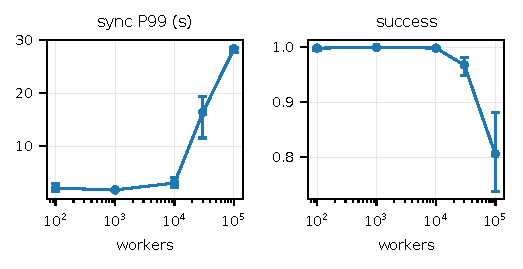
\includegraphics[width=\columnwidth]{figures/fig_scale}
\caption{Scalability (E18): sync P99 and success against population (log scale), mean with 95\% intervals; the two largest points use 3 seeds.}
\label{fig:scale}
\end{figure}

\begin{table}[t]
\caption{Scalability (E18): orchestrator and control-plane load.}
\label{tab:scale}
\centering\scriptsize
\resizebox{\columnwidth}{!}{% Generated by experiments/paper_tex.py; do not edit.
\begin{tabular}{rrrrrrr}
\toprule
\textbf{Workers} & \textbf{Seeds} & \textbf{Success (\%)} & \textbf{P99 (s)} & \textbf{Decide P99 (s)} & \textbf{Msg/s/worker} & \textbf{Orch. CPU (s/s)} \\
\midrule

100 & 10 & 99.8{\scriptsize$\pm$0.3} & 2.1{\scriptsize$\pm$0.8} & 0.10{\scriptsize$\pm$0.01} & 0.97{\scriptsize$\pm$0.04} & 0.000{\scriptsize$\pm$0.000} \\
1\,000 & 10 & 100.0{\scriptsize$\pm$0.1} & 1.7{\scriptsize$\pm$0.2} & 0.10{\scriptsize$\pm$0.01} & 0.74{\scriptsize$\pm$0.01} & 0.002{\scriptsize$\pm$0.000} \\
10\,000 & 10 & 99.8{\scriptsize$\pm$0.1} & 3.0{\scriptsize$\pm$0.9} & 0.48{\scriptsize$\pm$0.59} & 0.73{\scriptsize$\pm$0.01} & 0.021{\scriptsize$\pm$0.000} \\
30\,000 & 3 & 96.8{\scriptsize$\pm$1.6} & 16.4{\scriptsize$\pm$3.9} & 14.45{\scriptsize$\pm$11.95} & 0.74{\scriptsize$\pm$0.01} & 0.062{\scriptsize$\pm$0.000} \\
100\,000 & 3 & 80.6{\scriptsize$\pm$7.2} & 28.3{\scriptsize$\pm$0.5} & 29.83{\scriptsize$\pm$8.05} & 0.82{\scriptsize$\pm$0.03} & 0.207{\scriptsize$\pm$0.001} \\
\bottomrule
\end{tabular}
}
\end{table}

\subsection{Sensitivity to calibration (E24)}
\label{sec:res-calib}
Do conclusions depend on the measured values? We repeated the key comparison under the placeholder and the laptop-measured bundles (Table~\ref{tab:calibsens}).
\voss{}'s P99 is \CalSensVossPNinetynineMeas\,s with measured parameters against \CalSensVossPNinetyninePlc\,s with placeholders, but the simple baseline moves from
\CalSensSimplePNinetyninePlc\,s to \CalSensSimplePNinetynineMeas\,s: the advantage of planning \emph{grows} under the measured parameters. This shows that the main qualitative conclusion is not an artifact of the
placeholders; absolute values should not be read as predictions.

\begin{table}[t]
\caption{Calibration sensitivity (E24): placeholder versus laptop-measured parameters.}
\label{tab:calibsens}
\centering\scriptsize
\resizebox{\columnwidth}{!}{% Generated by experiments/paper_tex.py; do not edit.
\begin{tabular}{llrrrr}
\toprule
\textbf{Bundle} & \textbf{System} & \textbf{P50 (s)} & \textbf{P99 (s)} & \textbf{Met} & \textbf{Exposure} \\
\midrule

placeholder (C0 design) & VOSS & 0.429{\scriptsize$\pm$0.083} & 1.32{\scriptsize$\pm$0.11} & 0.984{\scriptsize$\pm$0.006} & 47{\scriptsize$\pm$4} \\
placeholder (C0 design) & simple baseline & 0.509{\scriptsize$\pm$0.095} & 3.89{\scriptsize$\pm$0.60} & 0.965{\scriptsize$\pm$0.010} & 53{\scriptsize$\pm$3} \\
measured (laptop) & VOSS & 0.239{\scriptsize$\pm$0.040} & 1.17{\scriptsize$\pm$0.25} & 0.978{\scriptsize$\pm$0.005} & 37{\scriptsize$\pm$4} \\
measured (laptop) & simple baseline & 0.266{\scriptsize$\pm$0.052} & 4.59{\scriptsize$\pm$0.65} & 0.954{\scriptsize$\pm$0.011} & 53{\scriptsize$\pm$3} \\
\bottomrule
\end{tabular}
}
\end{table}

\subsection{Scorecard}
\label{sec:res-score}
Of the hypotheses stated before the runs, \ScoreSupported{} are supported, \ScoreWeak{} weak, \ScoreInconclusive{} inconclusive and \ScoreRefuted{} refuted (Table~\ref{tab:score}).
The refuted and inconclusive entries are as informative as the supported ones: geo-clustering (H7), the simple baseline on homogeneous hosts (H11), and the
trust-establishment cost ratio of confidential VMs (H5) were wrong in the direction predicted, and the robust constraint, the MILP over greedy planning, caching and hedging
are inconclusive.

\begin{table*}[t]
\caption{Hypothesis scorecard. $\Delta$ rel.: paired relative change with 95\% bootstrap interval; verdict by the rules of Sec.~\ref{sec:method}. ``--'': cost-side information, no verdict.}
\label{tab:score}
\centering\scriptsize
% Generated by experiments/paper_tex.py; do not edit.
\begin{tabular}{lp{5.6cm}lp{2.2cm}rl}
\toprule
\textbf{H} & \textbf{Claim} & \textbf{Exp.} & \textbf{Cell} & \textbf{$\Delta$ rel. [95\% CI]} & \textbf{Verdict} \\
\midrule

H1 & MILP planner cuts sync P99 vs no planning & E04 & churn\_med & -54.6\% {\scriptsize[-105.6, -13.6]} & \textbf{supported} \\
H1 & MILP planner cuts sync P99 vs no planning & E04 & churn\_high & -60.2\% {\scriptsize[-96.8, -26.1]} & \textbf{supported} \\
H1 & ... and vs keep-alive TTL & E04 & churn\_med & -28.9\% {\scriptsize[-57.6, -8.3]} & \textbf{supported} \\
H1 & ... and vs keep-alive TTL & E04 & churn\_high & -57.9\% {\scriptsize[-117.5, -10.9]} & \textbf{supported} \\
H1 & donor memory held warm: MILP vs keep-alive TTL (cost side) & E04 & churn\_med & +112.3\% {\scriptsize[+90.7, +129.4]} & -- \\
H2 & f-robust plans keep success where non-robust collapse ($\alpha$=0.2 mixed) & E08 & mixed $\alpha$=0.2 & -0.1\% {\scriptsize[-0.3, +0.0]} & inconclusive \\
H3 & Pareto front has a knee; moderate exposure loses little latency & E23 &  & +0.5\%  & \textbf{supported} \\
H4 & progress detection beats heartbeat-only on success under $\alpha$=0.2 & E08 & mixed $\alpha$=0.2 & -3.2\% {\scriptsize[-4.3, -2.1]} & \textbf{supported} \\
H5 & appliance warm start $\approx$ Firecracker without attestation (L3) & E-CS1 (sim) &  & -2.0\%  & \textbf{supported} \\
H5 & appliance snapshot start $\approx$ Firecracker without attestation (L2) & E-CS1 (sim) &  & +2.5\%  & \textbf{supported} \\
H5 & CVM classes are 10-100x slower than the appliance to establish trust & E-CS1 (sim) &  & -92.7\%  & \textbf{refuted} \\
H6 & GDSF + P2P + HDD tier beat LRU without P2P/HDD (sync P99) & E09 &  & +3.1\% {\scriptsize[-2.7, +12.3]} & inconclusive \\
H6 & ... GDSF vs LRU alone & E09 &  & +1.8\% {\scriptsize[-0.1, +4.2]} & inconclusive \\
H7 & geo clusters reduce sync P99 vs one global scheduler (EU) & E05 & regions=[eu] & +16.5\% {\scriptsize[+10.8, +21.6]} & \textbf{refuted} \\
H7 & ... EU+NA & E05 & regions=[eu, na] & +16.6\% {\scriptsize[+5.2, +33.1]} & \textbf{refuted} \\
H7 & ... world & E05 & regions=[] & +4.7\% {\scriptsize[+1.2, +8.8]} & \textbf{refuted} \\
H8 & planner MILP beats greedy by $\geq$5\% sync P99 (high churn) & E04 & churn\_high & -2.5\% {\scriptsize[-5.8, +0.5]} & inconclusive \\
H9 & distribution-aware (quantile) beats expectation-only on P99 at high churn & E03 & churn\_high, name=blr & -2.8\% {\scriptsize[-5.3, -0.8]} & weak \\
H10 & accounting is off the critical path: settlement period 10 s vs 300 s & E13 & faults=[] & +1.5\% {\scriptsize[-0.2, +4.2]} & \textbf{supported} \\
H10 & ... receipt batch 0.2 s vs 5 s & E13 & faults=[] & -1.0\% {\scriptsize[-3.3, +1.0]} & \textbf{supported} \\
H11 & simple baseline matches VOSS when homogeneous, stable and benign & E10 & hw=C1 & +62.8\% {\scriptsize[+25.0, +111.5]} & \textbf{refuted} \\
H-FT1 & progress detection vs heartbeat-only: success with a black-holed scheduler & E15 & faults=sched\_blackhole & +3.2\% {\scriptsize[+2.7, +3.7]} & \textbf{supported} \\
H-FT3 & risk-proportional hedging ($\theta$=.3, 5\%) cuts sync P99 under $\alpha$=0.1 & E16 & mixed $\alpha$=0.1 & -13.3\% {\scriptsize[-32.5, +1.4]} & inconclusive \\
H-FT3 & ... at what extra-attempt cost & E16 & mixed $\alpha$=0.1 & +253.1\% {\scriptsize[+182.9, +332.3]} & -- \\
RQ15 & VOSS vs Lambda-like reference, sync P99 at 20 inv/s & E17 & rate=20 & +14.2\% {\scriptsize[+10.9, +18.1]} & -- \\
E12 & reputation tie-break (beta-decay) improves sync P99 vs no reputation & E12 &  & -2.4\% {\scriptsize[-4.4, -0.8]} & weak \\
E12 & ... and success rate & E12 &  & -0.0\% {\scriptsize[-0.0, +0.0]} & inconclusive \\
\bottomrule
\end{tabular}

\end{table*}

\section{Discussion}
\label{sec:discussion}

\medskip\noindent\textbf{What the evidence supports.}
The central design claim holds in simulation: treating trust and warm state as a planned, perishable resource beats reactive policies.
Planning cuts tail latency by half or more against no planning under churn, the lifecycle-aware placer and the planner are the two largest contributors in the ablation,
and progress-based detection is what keeps success high when owners omit. These are statements about mechanisms and are
supported by paired intervals. They hold across churn regimes and adversary fractions in the viability maps (Sec.~\ref{sec:res-viab}), not only at one operating point.

\medskip\noindent\textbf{What it does not.}
Four expected benefits did not materialize. (i)~Geo-clustering is slower than a single scheduler and holds several times the exposure. (ii)~The exact MILP
is not demonstrably better than a greedy planner, so the solver's cost (\MilpSolveS\,s per cluster) is justified only by the coverage guarantee, which we
could not show matters for \emph{success} (H2). (iii)~Caching sophistication and reputation tie-breaking change P99 by a few percent at most, and credit
under the current rules is extremely concentrated. (iv)~A commercial-style reference has lower latency, and \voss{} is cheaper per invocation only once the
fixed orchestrator tier is amortized over enough load. None of this contradicts the premise that volunteer hardware can serve latency-sensitive
functions at some SLO; it narrows which components earn their complexity. A simpler \voss{} without geo-clustering, reputation and tiered caches is the
version our evidence favors.

\medskip\noindent\textbf{Exposure is the price.}
Most latency gains are bought with exposure: planning, robustness and warm state all enlarge the set of hosts that hold a tenant's key. The simple baseline has about half
of \voss{}'s exposure, and the Pareto front shows that moderate robustness captures most of the benefit. We deliberately report exposure as a separate axis; a deployer
with high-sensitivity tenants would pick a lower $f$ and a higher exposure weight, accepting the latency cost shown in Fig.~\ref{fig:pareto}.

\medskip\noindent\textbf{Why the attestation argument matters.}
Every robustness result above uses omission and timing faults only. If attestation failed, for example through the physical attacks excluded in Sec.~\ref{sec:threat},
adversaries could forge results and read keys, and exposure would no longer be a proxy for risk. The design's honesty is conditional on attestation holding, and we
therefore treat liveness and owner notices as hints and verify progress.

\subsection{Threats to validity}
\label{sec:threats}
\begin{itemize}
\item \textbf{Simulation only.} No multi-machine deployment has validated the simulator end to end. Policies are the real code, but the world model (network, churn,
adversaries) is a model. We therefore interpret differences between designs, not absolute latencies.
\item \textbf{Calibration scope.} Calibration comes from one consumer laptop with a hard disk. Confidential-VM and DRTM parameters are literature values, and the laptop-measured
appliance runs in host mode. E24 shows the main comparison survives a change of bundle, but a different CPU, SSD or firmware could shift the absolute costs.
\item \textbf{Assumed workload and churn.} No public trace of consumer donation sessions exists; the churn shapes are assumed from availability studies and swept in E14.
The function catalogue follows SeBS but its sizes are assumed. The adversary model is omission and timing only, with a fixed menu of strategies. An adaptive adversary that learns the scheduler could do worse.
\item \textbf{Scale.} The two largest scalability points use three seeds and a cheaper simulator mode, and a $10^5$-worker deployment may behave differently.
\item \textbf{Statistics and selection.} Ten seeds give wide intervals for tail metrics; several comparisons are inconclusive rather than null. We ran many experiments, and a
verdict on a single comparison should be read with that in mind. Specifications were frozen before the final sweep, but pilots informed which cells to include (recorded in the decision log).
\item \textbf{Bibliography and prior numbers.} Literature parameters (for example confidential-VM startup) are quoted from the cited studies and are tagged for re-verification.
\end{itemize}

\subsection{Future work}
Validate on a small real testbed with end-to-end measurements (the first experiment in our plan, not yet run); measure confidential-VM hosts to replace literature parameters; shard
the orchestrator tier and re-measure scalability; revisit geo-clustering at larger populations and with shared trust across clusters; and study adaptive adversaries and
incentives given the observed credit concentration.

\section{Conclusion}
\label{sec:conclusion}
Attestation turns malicious volunteer owners into omission and timing faults, and what remains is the scheduling of a perishable resource: trust. A two-timescale design, a robust
slow-loop plan over trust and warm state plus a fast cost-based placer with progress-based failure detection, is viable in simulation in regimes where simple baselines are not
(\ViabAPThreeVoss{} of \ViabACells{} and \ViabBPThreeVoss{} of \ViabBCells{} cells at a 3\,s sync P99 target), cuts tail latency by \HOnePctNoneMed--\HOnePctNoneHigh\% against no planning, and keeps success at \VossSuccAlpha\% with 20\% omitting
owners. The advantage is not universal: on confidential-VM substrates at high load the simple baseline is the only viable system on the deadline-met criterion. Our paired, mechanically judged evaluation also shows what does not pay: geo-clustering, the exact solver over greedy planning, caching sophistication and reputation tie-breaking, and a
commercial-style reference remains faster. The design is better read as a small core (attestation, planned trust and warm state, progress detection) than as the full catalog of mechanisms we explored.
The next step is a real multi-machine testbed to validate the simulator, which this paper does not yet provide.


\bibliographystyle{IEEEtran}
\bibliography{refs}

\end{document}
